\documentclass{standalone}

\usepackage[english]{babel}
\usepackage[linesnumbered, ruled, vlined]{algorithm2e}

\usepackage{caption}

% to create listings

\usepackage{listings, lstautogobble}
\lstset{
  autogobble=true,
  frame=single,
}

\lstdefinelanguage{coq}[Objective]{Caml}{
  morekeywords={Structure, Definition, Inductive, list, return},
  sensitive=true
}

% to define font size

\usepackage{ulem}
\usepackage{moresize}
\usepackage{anyfontsize}

% to use tikz and its libraries

\usepackage{tikz-timing}
\usetikztiminglibrary[dual arrows]{clockarrows}

\usepackage{tikz}

\usetikzlibrary{backgrounds}
\usetikzlibrary{positioning, calc, arrows, shapes, automata, petri, patterns, decorations.markings}

% to use tikzmark, to place and refer to marks outside the current figure

\tikzset{every picture/.style={remember picture}}

% styles for transitions

\tikzset{transition/.append style={fill=black!20, thick}}
\tikzset{transition/.append style={fill=black!20, thick}}

% styles for test and inhib arcs.

\tikzstyle{test}=[pre, *-]
\tikzstyle{inhib}=[pre, o-]

% Arrow positioning in a path

\tikzset{->-/.style={decoration={
  markings,
  mark=at position #1 with {\arrow{>}}},postaction={decorate}}}

\tikzset{-<-/.style={decoration={
  markings,
  mark=at position #1 with {\arrow{<}}},postaction={decorate}}}

% to use colors

\usepackage{xcolor}

%%%%%%%%%%%%%%%%%%%%%%%%%%%%%%%%%%%%%%%%%%%%%%%%%%
%                  BEGIN DOCUMENT                %
%%%%%%%%%%%%%%%%%%%%%%%%%%%%%%%%%%%%%%%%%%%%%%%%%%

\begin{document}

% \tikzset{timing/font={\fontsize{80}{82}\selectfont}}

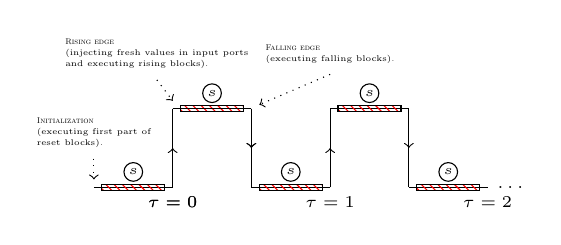
\begin{tikzpicture}
  
  % \timing[name=clock] {6{C}L};

  \coordinate (origin) at (0, 0);
  \coordinate (frelow) at ($(origin)+(1,0)$);
  \coordinate (frehigh) at ($(frelow)+(0,1)$);
  \coordinate (ffehigh) at ($(frehigh)+(1,0)$);
  \coordinate (ffelow) at ($(ffehigh)-(0,1)$);
  
  \draw (origin)  --
  node[draw, circle, anchor=south, yshift=2pt, inner sep=1pt] {\tiny $s$}
  node[pattern=north west lines, pattern color=red, draw, rectangle, minimum width=.8cm, inner sep=1pt] {}
  (frelow);
  \draw (frelow) edge[->-=.5] (frehigh);
  \draw (frehigh) --
  node[draw, circle, anchor=south, yshift=2pt, inner sep=1pt] {\tiny $s$}
  node[pattern=north west lines, pattern color=red, draw, rectangle, minimum width=.8cm, inner sep=1pt] {}
  (ffehigh);
  \draw (ffehigh) edge[->-=.5] (ffelow);
  \draw (frehigh) -- (ffehigh) edge[->-=.5] (ffelow);
  
  \draw (ffelow) --
  node[draw, circle, anchor=south, yshift=2pt, inner sep=1pt] {\tiny $s$}
  node[pattern=north west lines, pattern color=red, draw, rectangle, minimum width=.8cm, inner sep=1pt] {}
  ++ (1, 0)
  % tau = 1
  node[anchor=north] {\ssmall $\tau=1$} edge[->-=.5]++ (0,1);

  \draw (3, 1) --
  node[draw, circle, anchor=south, yshift=2pt, inner sep=1pt] {\tiny $s$}
  node[pattern=north west lines, pattern color=red, draw, rectangle, minimum width=.8cm, inner sep=1pt] {} ++ (1,0);
  
  \draw (4, 1) edge[->-=.5]++ (0,-1);
  
  \draw (4, 0) --
  node[draw, circle, anchor=south, yshift=2pt, inner sep=1pt] {\tiny $s$}
  node[pattern=north west lines, pattern color=red, draw, rectangle, minimum width=.8cm, inner sep=1pt] {} ++ (1,0)
  node[anchor=west]
  {\ssmall $\dots$} node[anchor=north] {\ssmall $\tau=2$};
  
  % tau = 0
  \node[anchor=north] at ($(frelow)$) {\ssmall $\tau=0$};

  %% Time markers
  
  % tau = 0
  \node[anchor=north] at ($(frelow)$) {\ssmall $\tau=0$};

  % Initialization
  \node (init) at ($(origin)+(0,.7)$) {
    \fontsize{3}{4}\selectfont
    \begin{tabular}{@{}l@{}}
      \textsc{Initialization} \\
      (executing first part of \\
      reset blocks). \\
    \end{tabular}
  };

  \draw (init) edge[->, dotted] ($(origin)+(0,.1)$);
  
  % Inj + RE
  \node (re) at ($(frehigh)+(-.2,.7)$) {
    \fontsize{3}{4}\selectfont
    \begin{tabular}{@{}l@{}}
      \textsc{Rising edge} \\
      (injecting fresh values in input ports \\
      and executing rising blocks). \\
    \end{tabular}
  };

  \draw ($(re.south)$) edge[->, dotted] ($(frehigh)+(0,.1)$);

  % FE
  \node (fe) at ($(ffehigh)+(1,.7)$) {
    \fontsize{3}{4}\selectfont
    \begin{tabular}{@{}l@{}}
      \textsc{Falling edge} \\
      (executing falling blocks). \\
    \end{tabular}
  };


  \draw ($(fe.south)$) edge[->, dotted] ($(ffehigh)+(.1,.05)$);

  % Stabilization phases
  % \node[draw, rectangle, minimum width=.8cm, inner sep=1pt] at ($(origin)+(.1,0)!.5!(frelow)-(.1,0)$) {};
  
\end{tikzpicture}

\end{document}
%%% Local Variables:
%%% mode: latex
%%% TeX-master: t
%%% End:
